\section{Method Evaluation} % on Synthetic and Real Data}
    \label{section:simu}
    \noindent
    \vspace{-1cm}
    \subsection{Synthetic data}
        \label{subsection:simu_param}
        \noindent
        A time series of $l = p + 1 = 20$ images is simulated. The covariance matrix is generated according to (\ref{Equation:cov_mat_struc}), where $\mathbf{\tilde{\Psi}}$ is simulated as a Toeplitz matrix i.e.,  $[ \mathbf{\tilde{\Psi}}]_{ij} = \rho^{|i-j|}$ with a coefficient correlation $\rho = 0.7$. %\in [ 0.5, 0.7, 0.9]$. 
        In the matrix $\mathbf{\tilde{\Psi}}$,  the coherence between the new image and the previous ones, $\boldsymbol{\gamma}$, corresponds to the last row and the scalar at $(l, l)$ position corresponds to the variance of the new image $\gamma_{l}$. We simulate linearly $l$ \acs{SAR} phases between $0$ and $2 \pi$, i.e., $\Delta_{i, i-1} = \theta_i - \theta_{i-1} = 2/l$ rad. The $n$ \acs{i.i.d} samples are then simulated as $\mathbf{\tilde{x}}^i \sim\mathcal{CN}(0, \tau_i \mathbf{\tilde{\Sigma}})$, where each $\tau_i$ is sampled according to a Gamma distribution $\tau \sim \Gamma(\nu, \frac{1}{\nu})$ with $\nu = 0.1$. %The case $\{\tau_i\}_{i=1}^n = 1 $ is equivalent to a Gaussian distributed samples.
        %\textcolor{blue}{The scale parameter  $v \in \mathbb{R}^+$ governs the tail of the distribution. As the value of $v$ increases ($v \rightarrow \infty$), the distribution approaches a Gaussian distribution, whereas a smaller value of $v$ results in a more heavy-tailed distribution.}
        %\textcolor{blue}{Heavy-tailed distributions capture heterogeneities by modeling a wider range of variability in the data. This flexibility makes them suitable for datasets with diverse or irregular behavior, specifically, for urban areas which is known to include spatial heterogeneity.}
        %\textcolor{blue}{
        The scale parameter  $v \in \mathbb{R}^+$ governs the tail of the distribution. When the value of $\nu$ is small (e.g., $\nu = 0.1$), the simulated data become highly heterogeneous, which is desirable as it aligns with the characteristics of urban areas in the real world. However, if the data are Gaussian ($v \rightarrow \infty$), similar to natural environments, the method produces results identical to those of a Gaussian model based approach, since in covariance matrix estimation, non-Gaussian estimators perform similarly to Gaussian estimators under a Gaussian distribution \citep{pascal2008empirical, harari2008use}.%}
        We compare our results with those obtained from other state-of-the-art approaches: %$2$-pass \acs{InSAR} designated hereinafter by $2$p-\acs{InSAR}, which is equivalent to generate an interferogram between $2$ images, 
        classic \acs{PL} \citep{cao2015mathematical} and \acs{MLEPL} \citep{vu2023robust}. We consider the \ac{MSE} which is computed using $1000$ Monte Carlo trials.
        %An additional comparison is presented to prove the effectiveness of the non gaussian model assumption. 
    \vspace{0.5em}
    \subsubsection{Comparison with offline approaches}
       \label{subsubsection:comp_offline}
       \vspace{-1em}
        \begin{figure}[H]
        \centering
        \begin{subfigure}[b]{0.45\columnwidth} 
            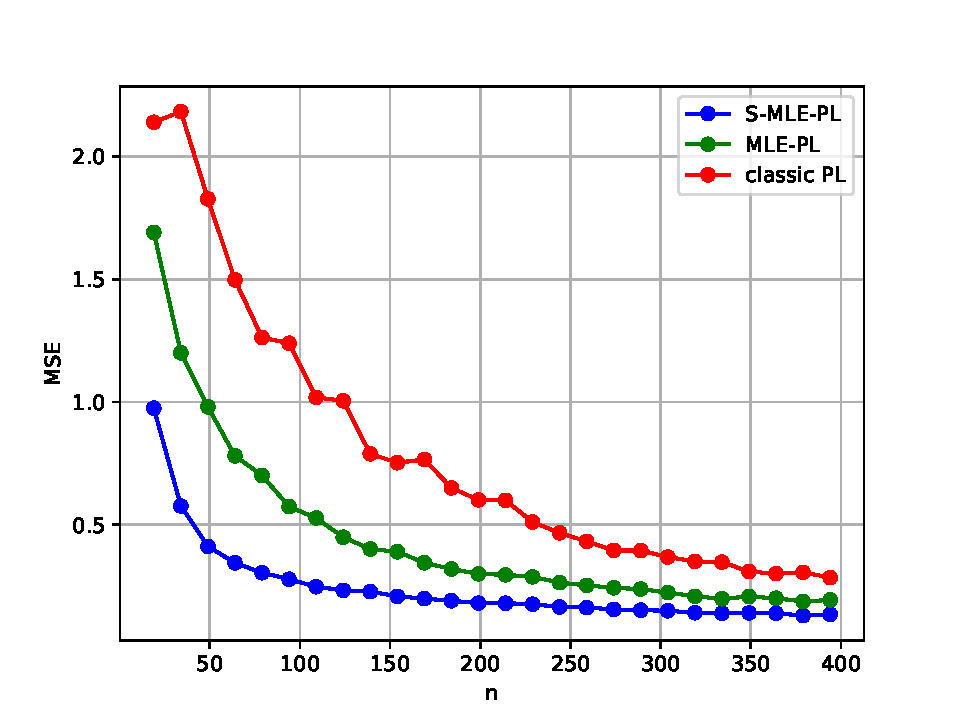
\includegraphics[width=\linewidth, trim = 0cm 0cm 0cm 1.3cm, clip]{images/gamma_0.1/rho_0.7_p+1_20_('ScaledGaussian', 0.1)_n>=19maxphase=1_init_w=1_papierMSE_date20.pdf}     
            \caption{Comparison with offline approaches}
            \label{fig:MSE_simu}
        \end{subfigure}
        %\hfill % Espace horizontal entre les colonnes
        \begin{subfigure}[b]{0.45\columnwidth} 
            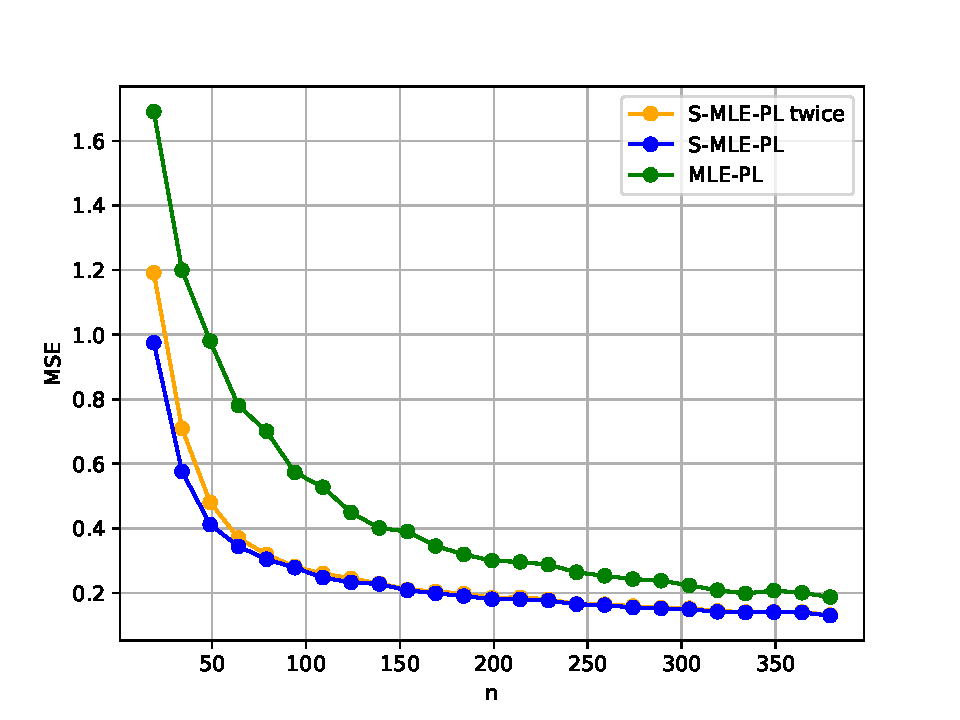
\includegraphics[width=\linewidth, trim = 0cm 0cm 0cm 1.3cm, clip]{images/seq_integration/MSE_rho_0.7_date_20.pdf} 
            \caption{Sequential integration of several new images}
            \label{fig:multiple_bloc}
        \end{subfigure}
        \caption{\small \acs{MSE} of phase difference estimation between the $1^{\text{st}}$ and $20^{\text{th}}$ (last) dates for $l = 20$  with respect to increasing sample size ($n$) using $1000$ Monte Carlo trials.}
    \end{figure}
    \vspace{-1em}
    %\vspace{-0.2cm}
    \noindent
        Fig. \ref{fig:MSE_simu} represents the \acs{MSE} of phase estimates for a sample size $n = 64$ when $n$ increases. As foreseen, the larger the sample size, the better the performances are in terms of \acs{MSE} for all approaches. Offline approaches require operations on large matrices, such as matrix inversion which is sensitive to the samples size. The sequential approach shows better results particularly on small sample size. For low sample support %\textcolor{blue}{
        ($n < 100$)%}
        , \acs{SMLEPL} shows better performance than classic \acs{PL} and \acs{MLEPL}. 
        %In this paper, we focus on the comparison between the sequential and the offline approach, highlighting that a variation of the parameter $\nu$ is possible, which was already presented in \citep{vu2023robust}.
        In this paper, we compare the sequential and offline approaches, highlighting the potential for parameter $\nu$ variation. % as previously discussed in \citep{vu2023robust}.
        %\textcolor{blue}{Heavy-tailed distributions capture heterogeneities by modeling a wider range of variability in the data. This flexibility makes them suitable for datasets with diverse or irregular behavior, specifically, for urban areas which is known to include spatial heterogeneity.}
        
    \vspace{0.5em}
    \subsubsection{Sequential integration of several new images}
        \label{subsubsection:seq_integration}
        %\begin{enumerate}
        %    \item The offline method \acs{sgMLEPL} where we directly process the $p+2$ images. 
        %    \item The partial sequential method, where the $p+1$ past phases are computed using the offline method 
        %    \item The full sequential method, where only $p$ phases are calculated using the offline approach, the $p+1$ and $p+2$ phases are estimated sequentially \acs{SsgMLEPL} twice
            %\yysup{the $p+1$ past phases consist of $p$ phases calculated using the offline approach and $(p+1)^{\text{th}}$ phase calculated using the sequential method}.
        %\end{enumerate}
       % \vspace{-0.3cm}
        %\begin{figure}[H]
        %    \centering
        %    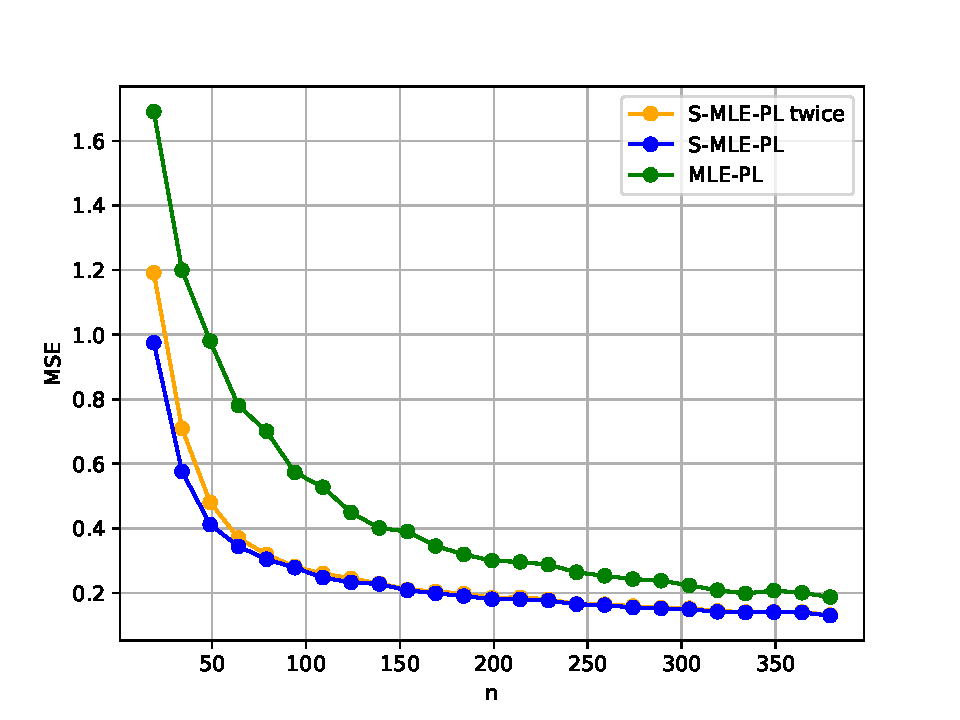
\includegraphics[width=5cm, trim = 0cm 0cm 0cm 1.3cm, clip]{images/seq_integration/MSE_rho_0.7_date_20.pdf}
        %    \vspace{-10pt}
        %    \caption{\small \ac{MSE} on $w_{\theta_{l}}$ with increasing $n$, $l = 20$, $\rho=0.7$ using $1000$ Monte Carlo trials.}
        %    \label{fig:multiple_bloc}
        %\end{figure}
        %\vspace{-0.3cm}
        \noindent
        %This approach involves adding a new image each time. It is interesting to investigate the error propagation of the estimated phase. Let's consider a block of $p$ images (representing the past). Initially, a new image is added (indexed as $p+1$) and we employ our sequential approach to estimate the $(p+1)^{\text{th}}$ phase using the $p$ past images. Subsequently, we add another new image (indexed as $p+2$). At this point, we aim to compare the estimations of the $(p+2)^{\text{th}}$ phase in three distinct manners. 
        %First, the offline method \acs{MLEPL}, which directly processes all $(p+2)$ images. Second, the partial sequential method, where the $(p+1)$ preceding phases are calculated using the offline method. Finally, the full sequential method, where only $p$ phases are computed using the offline approach, and the $(p+1)^{\text{th}}$ and $(p+2)^{\text{th}}$ phases are estimated sequentially with \acs{SMLEPL} twice. 
        %We demonstrate that even after two additions of single new images, our approach continues to outperform the offline approach. Moreover, it performs equivalently to adding one observation at a time and applying the offline approach on the past block (Fig. \ref{fig:multiple_bloc}).
        %This approach involves adding a new image each time and investigating error propagation in the estimated phase. We consider a block of \normalsize \( p \) images (the past) and add a new image, indexed as \normalsize \( p+1 \). We then use our sequential method to estimate the \normalsize \((p+1)^{\text{th}}\) phase with these \normalsize \( p \) images. After adding another new image (indexed as \normalsize \( p+2 \)), we compare the \normalsize \((p+2)^{\text{th}}\) phase estimations in three ways: (a) the offline method \acs{MLEPL} processing all \normalsize \( (p+2) \) images, (b) the partial sequential method, where the \normalsize \((p+1)\) phases are calculated offline and (c) the full sequential method, estimating the \normalsize \((p+1)\) and \normalsize \((p+2)\) phases sequentially with \normalsize \acs{SMLEPL} after computing \normalsize \( p \) phases offline. We show that our approach outperforms the offline method even after two new images, performing comparably to adding one observation at a time and applying the offline method on the past block (Fig. \ref{fig:multiple_bloc}).
    %\textcolor{blue}{
    We compare $3$ setups: (a) offline processing (\acs{MLEPL}): processing the entire set together, (b) partial sequential processing (\acs{SMLEPL}): the last phase is estimated with the proposed approach and (c) full sequential processing (\acs{SMLEPL} twice): the last $2$ images are added sequentially and the \acs{SMLEPL} is used twice. %}
    %\begin{enumerate}
    %    \item Offline Processing: processing the entire set together.
    %    \item Partial Sequential Processing: the last phase is estimated the proposed approach
        %the phases for the previous images are calculated offline, while the new image’s phase is estimated using this prior information.
    %    \item Full Sequential Processing: the last $2$ images are added sequentially and the \acs{SMLEPL} is used twice sequentially
        %This method estimates the phases sequentially, first calculating the phases for the previous images offline and then estimating the phases for the newly added images one after the other.
    %\end{enumerate}
    %\textcolor{blue}{We show that our approach outperforms the offline method even after two new images, performing comparably to adding one observation at a time and applying the offline method on the past block (Fig. \ref{fig:multiple_bloc}).}
    %\textcolor{blue}{
    We show that the full sequential processing outperforms the offline processing (\acs{MLEPL}), and performs comparably to adding one observation at a time (Fig. \ref{fig:multiple_bloc}).%}
    %even after two new images added sequentially
    